% LaTeX Report Template - customizing page format
%
% LaTeX document uses 10-point fonts by default.  To use
% 11-point or 12-point fonts, use \documentclass[11pt]{report}
% or \documentclass[12pt]{report}.

\documentclass[notitlepage]{article}


\usepackage{amsmath}
\usepackage{amssymb}
\usepackage{graphicx}
\usepackage{pdflscape}
\usepackage{multicol}
% Set width of the text - What is left will be the right margin.
\setlength{\oddsidemargin}{-0.25in}
% In this case, right margin is 8.5in - 1.25in - 6in = 1in.
\setlength{\textwidth}{6in}

% Set top margin - The default is 1 inch, so the following 
% command sets a 0.75-inch top margin.
\setlength{\topmargin}{-0.75in}

% Set height of the text - What is left will be the bottom margin.
% In this case, bottom margin is 11in - 0.75in - 9.5in = 0.75in
\setlength{\textheight}{19.5in}

% Set the beginning of a LaTeX document
\usepackage{Sweave}
\begin{document}
\input{tutorial-concordance}

\begin{flushleft} 
synDss Tutorial \\
Peter Chi and Vladimir Minin \\
\end{flushleft}

Objective: This is a tutorial to illustrate the use of the synDss package in {\tt{R}}. 

\begin{itemize}
\item The first
step is to download and install PAML, from:  
{\tt{http://abacus.gene.ucl.ac.uk/software/paml.html}}. 
\begin{itemize}
\item The two programs we need
from this software package are {\tt{codeml}} and {\tt{evolver}}. 
\begin{itemize}
\item For {\tt{codeml}}, the included MS Windows executable {\tt{codeml.exe}} will work as is on Windows,
and on Linux/Mac, one can compile {\tt{codeml.c}} following the PAML installation instructions.
\item For {\tt{evolver}}, we need
to compile it in a slightly different way in order to allow for variable dN/dS rates at
each site (i.e. the M3 model). Essentially, we need to go to the PAML subdirectory that contains {\tt{evolver.c}},
and type:
\begin{verbatim}
gcc -O4 -DCodonNSsites -o evolverNSsites evolver.c tools.c -lm
\end{verbatim}
This is assuming that a gcc compiler is installed on your machine, e.g. through RTools if you are using Windows.
See 
\begin{verbatim}
petrov.stanford.edu/software/src/paml3.15/Technical/Simulation/Codon/CodonSimulation.txt
\end{verbatim} 
for more details.

\end{itemize}
\item The {\tt{codeml}} and {\tt{evolverNSsites}} executables should then be placed in a folder of 
local programs pointed to by your PATH variable,
so that they can be run from any directory. See the PAML installation instructions for more details. Alternatively,
if this cannot be successfully performed, one will need to specify the directory where the PAML programs
are located when running certain functions (see below).

\end{itemize}


\item Next, we need to open {\tt{R}}, and install and load the {\tt{synDss}} package:
\begin{Schunk}
\begin{Sinput}
> #install.packages("synDss", repos="http:/R-Forge.R-project.org")
> library(synDss)
\end{Sinput}
\end{Schunk}

\item Now, let us try to calculate the original and synonymous Dss statistics from a DNA sequence
alignment. First, we will read in the fasta file for a sequence alignment of 18 salmonella sequences included
in the package:

\begin{Schunk}
\begin{Sinput}
> salmonella<-fasta.to.alignment(system.file("seqdata/Salmonella_fimH_aligned-18alleles.txt",package="synDss"))
> 
\end{Sinput}
\end{Schunk}

\item Now, let us calculate the Dss statistic for this dataset, with a window size of 105 nucleotides,
and step size of 9 nucleotides:

\begin{Schunk}
\begin{Sinput}
> dss.stat<-calc.Dss(salmonella, l=270, m=9)
> 
\end{Sinput}
\end{Schunk}

\item We can also calculate the synonymous Dss statistic (for a dataset of this size, this will take about 5 minutes):

\begin{Schunk}
\begin{Sinput}
> syn.stat<-calc.Dss.syn(salmonella, l=270, m=9,syn.matrix=regist.synonym())
> 
\end{Sinput}
\end{Schunk}

\item To look at our statistic landscapes, we can plot them:
\begin{Schunk}
\begin{Sinput}
> m<-9
> l<-270
> length<-dim(as.matrix.alignment(salmonella))[2]
> n.windows<-((length-(2*l))/m+1)
> index<-c(1:n.windows)
> title<-"sal18.pdf"
> pdf(title,height=4,width=8)
> max<-max(c(dss.stat,syn.stat),na.rm=T)
> plot(dss.stat~index,type="l",xlab="window number",ylab="",ylim=c(0,max),lty=2)
> lines(syn.stat~index,type="l")
> legend("topright",c("Original Dss","Synonymous Dss"),lty=c(2,1))
> dev.off()
\end{Sinput}
\begin{Soutput}
null device 
          1 
\end{Soutput}
\begin{Sinput}
> 
> 
\end{Sinput}
\end{Schunk}


\par Here is the landscape plot, with a window size of 540 and step size of 9:

\begin{figure}[ht]
\begin{center}
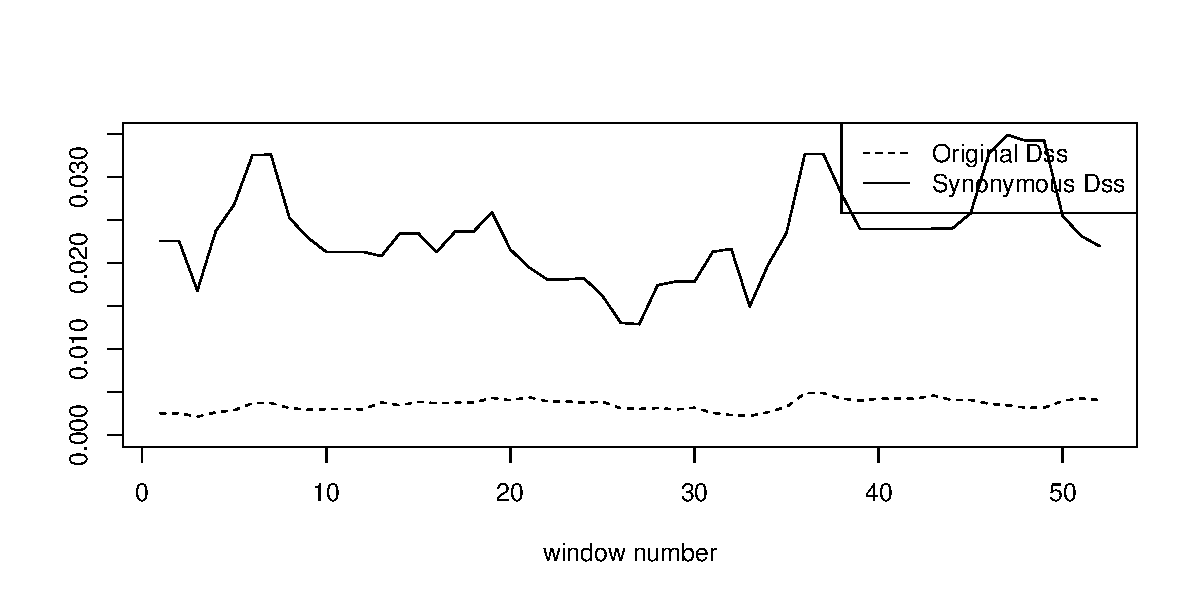
\includegraphics[width=\textwidth]{sal18.pdf}
\caption{Landscape plot for salmonella sequence alignment}
\label{fig:tree}
\end{center}
\end{figure}

\item Now, we need to obtain a statistical significance threshold in order to obtain
a p-value. We will do this through parametric bootstrap, as follows (later will up B; right
now just seeing if it works):

\begin{Schunk}
\begin{Sinput}
> null.dss<-calc.null.pboot(salmonella,B=1,270,9)